\documentclass{standalone}
\usepackage{pgfplots}
\pgfplotsset{compat=1.16}
\begin{document}
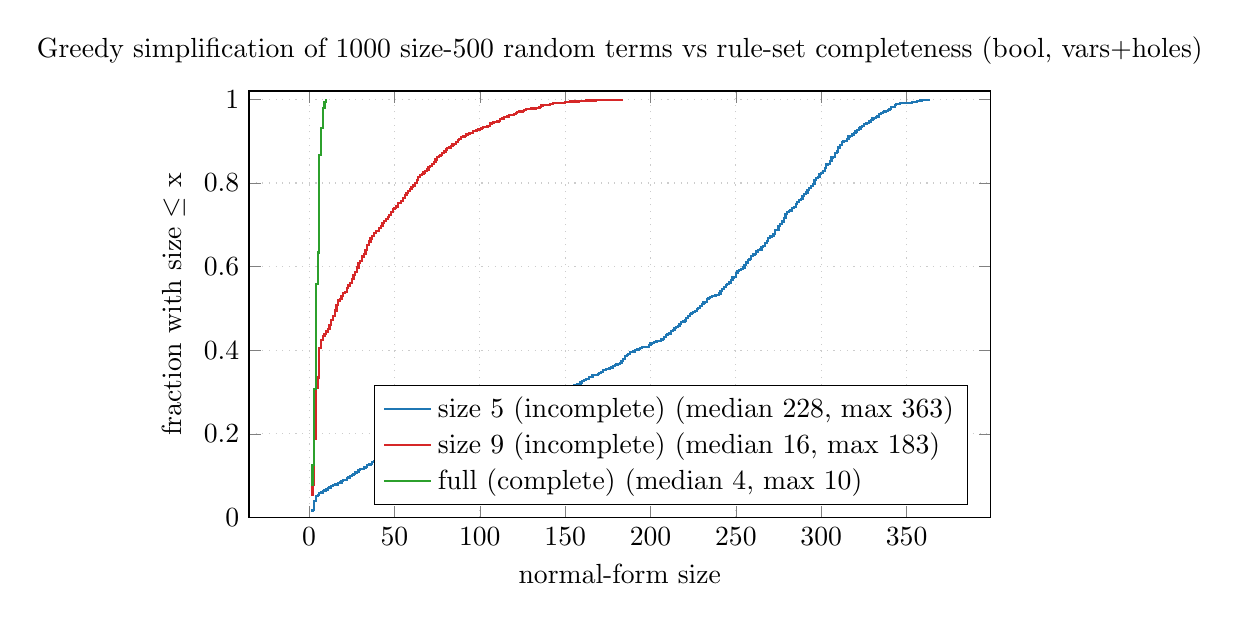
\begin{tikzpicture}
  \begin{axis}[
      width=11cm, height=7cm,
      xlabel={normal-form size}, ylabel={fraction with size $\leq$ x},
      title={Greedy simplification of 1000 size-500 random terms vs rule-set completeness (bool, vars+holes)},
      ymin=0, ymax=1.02, grid=both, grid style={dotted, gray!40},
      legend pos=south east, legend cell align=left,]
    \definecolor{c0}{HTML}{1f77b4}
    \addplot[color=c0, thick, const plot] coordinates {(1,0.0150) (2,0.0190) (3,0.0390) (4,0.0520) (5,0.0540) (6,0.0590) (7,0.0600) (8,0.0630) (9,0.0650) (10,0.0670) (11,0.0710) (12,0.0720) (13,0.0750) (14,0.0770) (15,0.0790) (17,0.0820) (18,0.0840) (19,0.0870) (20,0.0890) (21,0.0900) (22,0.0950) (23,0.0960) (24,0.0990) (25,0.1010) (26,0.1040) (27,0.1080) (28,0.1090) (29,0.1140) (30,0.1160) (31,0.1170) (32,0.1200) (33,0.1210) (34,0.1250) (35,0.1270) (36,0.1290) (37,0.1330) (38,0.1340) (39,0.1380) (40,0.1390) (41,0.1430) (42,0.1460) (43,0.1470) (44,0.1480) (46,0.1510) (47,0.1550) (48,0.1580) (50,0.1600) (51,0.1610) (53,0.1620) (54,0.1640) (55,0.1660) (56,0.1670) (57,0.1690) (61,0.1710) (62,0.1720) (63,0.1740) (64,0.1760) (65,0.1780) (66,0.1790) (68,0.1820) (69,0.1860) (70,0.1890) (71,0.1900) (73,0.1930) (74,0.1950) (75,0.1960) (76,0.1980) (77,0.2000) (81,0.2030) (83,0.2050) (84,0.2070) (86,0.2080) (87,0.2090) (90,0.2120) (91,0.2140) (92,0.2150) (93,0.2160) (94,0.2180) (95,0.2210) (96,0.2220) (97,0.2230) (98,0.2250) (99,0.2260) (100,0.2290) (101,0.2320) (102,0.2340) (103,0.2360) (105,0.2370) (106,0.2380) (107,0.2390) (108,0.2400) (109,0.2410) (110,0.2440) (111,0.2470) (113,0.2510) (114,0.2540) (116,0.2570) (117,0.2580) (120,0.2590) (121,0.2620) (122,0.2630) (123,0.2650) (124,0.2670) (125,0.2700) (128,0.2710) (130,0.2720) (131,0.2740) (132,0.2780) (133,0.2810) (134,0.2830) (135,0.2840) (137,0.2850) (139,0.2870) (140,0.2900) (141,0.2910) (142,0.2930) (143,0.2940) (144,0.2950) (145,0.3000) (146,0.3010) (147,0.3050) (148,0.3060) (149,0.3090) (151,0.3100) (153,0.3110) (154,0.3120) (155,0.3160) (156,0.3170) (157,0.3190) (158,0.3200) (159,0.3230) (160,0.3270) (161,0.3290) (162,0.3310) (164,0.3360) (165,0.3370) (166,0.3400) (168,0.3410) (169,0.3440) (170,0.3460) (171,0.3490) (172,0.3520) (173,0.3530) (174,0.3550) (176,0.3570) (177,0.3590) (178,0.3620) (179,0.3640) (180,0.3660) (181,0.3670) (182,0.3700) (183,0.3750) (184,0.3790) (185,0.3860) (186,0.3880) (187,0.3920) (188,0.3950) (189,0.3960) (190,0.3970) (191,0.4010) (192,0.4020) (193,0.4040) (194,0.4050) (195,0.4070) (196,0.4080) (199,0.4120) (200,0.4160) (201,0.4180) (202,0.4190) (203,0.4210) (204,0.4220) (205,0.4230) (206,0.4260) (207,0.4270) (208,0.4310) (209,0.4360) (210,0.4390) (211,0.4400) (212,0.4460) (213,0.4480) (214,0.4530) (215,0.4550) (216,0.4580) (217,0.4620) (218,0.4680) (219,0.4690) (220,0.4710) (221,0.4770) (222,0.4820) (223,0.4870) (224,0.4890) (225,0.4920) (226,0.4940) (227,0.4990) (228,0.5020) (229,0.5060) (230,0.5100) (231,0.5140) (232,0.5150) (233,0.5230) (234,0.5250) (235,0.5270) (236,0.5290) (238,0.5330) (240,0.5360) (241,0.5420) (242,0.5470) (243,0.5510) (244,0.5560) (245,0.5590) (246,0.5620) (247,0.5680) (248,0.5740) (249,0.5760) (250,0.5840) (251,0.5900) (252,0.5920) (253,0.5940) (254,0.5980) (255,0.6030) (256,0.6100) (257,0.6150) (258,0.6180) (259,0.6260) (260,0.6290) (261,0.6310) (262,0.6360) (263,0.6400) (264,0.6410) (265,0.6460) (266,0.6500) (267,0.6560) (268,0.6610) (269,0.6690) (270,0.6720) (271,0.6730) (272,0.6780) (273,0.6870) (274,0.6880) (275,0.6970) (276,0.7010) (277,0.7080) (278,0.7160) (279,0.7250) (280,0.7300) (281,0.7330) (282,0.7340) (283,0.7410) (284,0.7430) (285,0.7490) (286,0.7540) (287,0.7590) (288,0.7620) (289,0.7690) (290,0.7730) (291,0.7770) (292,0.7840) (293,0.7880) (294,0.7920) (295,0.7980) (296,0.8070) (297,0.8110) (298,0.8140) (299,0.8210) (300,0.8240) (301,0.8280) (302,0.8350) (303,0.8440) (304,0.8460) (305,0.8530) (306,0.8610) (307,0.8620) (308,0.8720) (309,0.8750) (310,0.8850) (311,0.8900) (312,0.8980) (313,0.9000) (314,0.9010) (315,0.9050) (316,0.9110) (317,0.9120) (318,0.9160) (319,0.9200) (320,0.9230) (321,0.9270) (322,0.9300) (323,0.9330) (324,0.9360) (325,0.9410) (326,0.9420) (327,0.9440) (328,0.9470) (329,0.9510) (330,0.9540) (331,0.9560) (332,0.9570) (333,0.9590) (334,0.9640) (335,0.9670) (336,0.9690) (337,0.9710) (338,0.9730) (339,0.9740) (340,0.9760) (341,0.9810) (343,0.9860) (344,0.9880) (345,0.9890) (346,0.9910) (352,0.9920) (353,0.9930) (355,0.9940) (356,0.9960) (358,0.9970) (359,0.9990) (363,1.0000)};
    \addlegendentry{size 5 (incomplete) (median 228, max 363)}
    \definecolor{c1}{HTML}{d62728}
    \addplot[color=c1, thick, const plot] coordinates {(1,0.0540) (2,0.0770) (3,0.1870) (4,0.3090) (5,0.3350) (6,0.4060) (7,0.4240) (8,0.4350) (9,0.4380) (10,0.4450) (11,0.4510) (12,0.4610) (13,0.4720) (14,0.4820) (15,0.4950) (16,0.5090) (17,0.5190) (18,0.5230) (19,0.5290) (20,0.5370) (21,0.5390) (22,0.5490) (23,0.5550) (24,0.5610) (25,0.5700) (26,0.5800) (27,0.5870) (28,0.5980) (29,0.6090) (30,0.6140) (31,0.6240) (32,0.6300) (33,0.6390) (34,0.6520) (35,0.6600) (36,0.6670) (37,0.6730) (38,0.6810) (39,0.6860) (41,0.6930) (42,0.6980) (43,0.7050) (44,0.7100) (45,0.7140) (46,0.7180) (47,0.7230) (48,0.7300) (49,0.7370) (50,0.7410) (51,0.7440) (52,0.7520) (53,0.7530) (54,0.7570) (55,0.7640) (56,0.7720) (57,0.7760) (58,0.7800) (59,0.7860) (60,0.7910) (61,0.7940) (62,0.7990) (63,0.8080) (64,0.8150) (65,0.8190) (66,0.8220) (67,0.8250) (68,0.8280) (69,0.8320) (70,0.8380) (71,0.8400) (72,0.8450) (73,0.8500) (74,0.8560) (75,0.8630) (76,0.8640) (77,0.8670) (78,0.8720) (79,0.8750) (80,0.8800) (81,0.8830) (82,0.8850) (83,0.8890) (84,0.8920) (85,0.8940) (86,0.8980) (87,0.9020) (88,0.9050) (89,0.9090) (90,0.9110) (91,0.9120) (92,0.9160) (93,0.9180) (94,0.9190) (95,0.9200) (96,0.9240) (97,0.9250) (98,0.9260) (99,0.9280) (100,0.9290) (101,0.9320) (102,0.9340) (104,0.9350) (105,0.9360) (106,0.9420) (107,0.9430) (108,0.9450) (109,0.9460) (110,0.9470) (111,0.9490) (112,0.9530) (113,0.9540) (114,0.9580) (116,0.9590) (117,0.9620) (118,0.9630) (120,0.9640) (121,0.9670) (122,0.9700) (123,0.9710) (125,0.9730) (126,0.9740) (127,0.9760) (129,0.9770) (130,0.9780) (133,0.9790) (134,0.9800) (135,0.9810) (136,0.9850) (137,0.9860) (139,0.9870) (141,0.9880) (143,0.9910) (146,0.9920) (150,0.9940) (153,0.9950) (158,0.9960) (162,0.9970) (168,0.9980) (173,0.9990) (183,1.0000)};
    \addlegendentry{size 9 (incomplete) (median 16, max 183)}
    \definecolor{c2}{HTML}{2ca02c}
    \addplot[color=c2, thick, const plot] coordinates {(1,0.0780) (2,0.1260) (3,0.3080) (4,0.5590) (5,0.6340) (6,0.8670) (7,0.9310) (8,0.9790) (9,0.9930) (10,1.0000)};
    \addlegendentry{full (complete) (median 4, max 10)}
  \end{axis}
\end{tikzpicture}
\end{document}
